\documentclass{article}
\usepackage[utf8]{inputenc}
\usepackage{graphicx}
\usepackage{multirow}
\usepackage{mathtools}
\usepackage[table,xcdraw]{xcolor}
\usepackage[T1]{fontenc} %żeby błedu \k command unavailable nie wywalało


\title{Kulawy Kustosz}
\author {Weronka Hilaszek\\ Zuzanna Makowska\\ Mateusz Mirecki\\ Wiktor Prosowicz\\ Karolina Surówka\\ Łukasz Zawadzki}

\date{2021/2022}

\begin{document}

\maketitle
\newpage

\section{Zuzanna Makowska}
\label{sec:zmakowska}

Here is a photo of my pet.

\begin{figure}[htbp]
    \centering
    
\includegraphics[width=0.5\textwidth]{Pictures/1_ZMakowska_picture.jpg}
    \caption{This is Bravo.}
    \label{fig:Bravo}
   
\end{figure}

\vspace{1.0cm}



An example of math equation:
$ \ a^2+b^2=c^2 \ $

Another one:
$ \ \binom{n}{k}=\frac{n!}{k!(n-k)!} \ $
\vspace{1cm}

\setlength{\parindent}{10ex}
 {Lorem ipsum dolor sit amet, consectetur adipiscing elit. Cras blandit ultrices dui eget dignissim. Suspendisse malesuada quis ipsum bibendum euismod. \textbf{In mollis luctus} ex, ut placerat risus consequat quis. Ut elementum sed tellus eget venenatis. Phasellus eget sapien porta, congue urna id, congue est. Maecenas in consectetur enim, et vulputate nibh. Curabitur maximus vulputate viverra. \underline{Donec sed nibh pulvinar, ultricies erat sit amet, imperdiet quam.} Integer gravida, dui non dictum tempus, ipsum eros tincidunt velit, et eleifend nunc ex quis mauris. Quisque quis nulla vitae tortor rutrum interdum. Etiam pulvinar suscipit nisl, et placerat tellus suscipit non. \textbf{Vestibulum leo orci, malesuada ut orci in, aliquam tincidunt nisl}. Cras massa erat, consequat eget lobortis nec, vulputate a ligula. Curabitur dui arcu, ultrices non malesuada at, consequat quis nisl.}.\par
\setlength{\parindent}{10ex}
 {Suspendisse sed urna in augue ultrices finibus. Pellentesque habitant morbi tristique senectus et netus et malesuada fames ac turpis egestas. \textit{Aliquam erat volutpat. Vivamus in placerat justo}. Sed ultrices, massa eget vehicula accumsan, ligula elit ultricies ex, sit amet commodo justo quam eu lacus. Morbi at elementum odio. Morbi a hendrerit nisi. Aliquam erat volutpat. Suspendisse accumsan vestibulum suscipit. Pellentesque vitae nisi ut lectus volutpat rutrum sed non justo.}
 

 
 \vspace{1.0cm}
    \begin{table}[htbp]
\centering

\begin{tabular}{||c |c| c||} 
 \hline \hline
 \textbf{month} & \textbf{days} & \textbf{season} \\  \hline\hline

 January & 31 & \multirow{3}{*}{winter} \\

 February & 28/29 &  \\

 March & 31 &   \\ \hline

 April & 30 & \multirow{3}{*}{spring}\\ 
 
 May & 31 & \\ 

 June & 30 & \\ \hline

 July & 31 & \multirow{3}{*}{summer} \\

 August & 31 &  \\

 September & 30 & \\ \hline

 October & 31 & \multirow{3}{*}{autumn}\\

 November & 30 & \\

 December & 31 &\\ \hline \hline

 
\end{tabular}


\caption{Months}
\label{tab:tab_months}

\end{table}
 Months in order (as presented in table \ref{tab:tab_months}):
\begin{enumerate}
    \item January
    \item February
    \item March
    \item April
    \item May
    \item June
    \item July
    \item August
    \item September
    \item October
    \item November
    \item December
    
\end{enumerate}

\vspace{2.0cm}
Seasons of the year:

\begin{itemize}
\renewcommand{\labelitemi}{$-$}
    \item Spring
    \item Summer
    \item Autumn
    \item Winter
\end{itemize}






 







\newpage

\section{Mirecki}
\label{sec:mmirecki}

Tu jest mój rozdział: 

\vspace{1cm}


Wstawione zdjecie zgody (patrz Figure~\ref{fig:pogodzenie})

\begin{figure}[htbp]
    \centering
    
\includegraphics[width=1\textwidth]{Pictures/1_MM.jpg}
    \caption{Pogodzone podejścia do wychowania}
    \label{fig:pogodzenie}
\end{figure}


Table~\ref{tab:sounds_of_motor} ukazuje onomatopeje dźwięku slinika na przestrzeni czasu!
    \begin{table}[htbp]
\centering
\begin{tabular}{|c| c c c|} 
    \hline
    Dźwięk auta & pierwsze 5s & kolejne 5s & dalsza jazda \\  
    \hline
    Przy odpalaniu & bulbulbul & łutututu & whmmm \\ 
    \hline
    Nagrzany & whmm & ziuu & ziuuuuum \\
    \hline
\end{tabular}
\label{tab:sounds_of_motor}
\caption{Tak się to kształtuje na przestrzeni czasu}
\end{table}



Pewna ciekawa funkcja:
\begin{align*}
  f(x) &= x^2\\
\end{align*}

A tu kolejna:
$   F(x) = \int^a_b \frac{1}{3}x^3 $

\vspace{1cm}

Lista liczb numerowanych
\begin{enumerate}
  \item 4
  \item 4
  \item 44
  \item 204
\end{enumerate}
\vspace{1cm}
Lista czegoś ale z punktorów

\begin{itemize}
\renewcommand{\labelitemi}{$>$}
    \item dzis
    \item jutro
    \item czegos
    \item brak
\end{itemize}




\setlength{\parindent}{10ex}
This is the text in first \underline{paragraph}. This is the text in first 
paragraph. This is the text in first paragraph. \par

\vspace{1cm}


\noindent %The next paragraph is not indented
Some of the \textbf{greatest} discoveries in \underline{science} were made by \textbf{\emph{accident}}.
This is the text in second paragraph.





\newpage

\section{Karolina Surówka}
\label{seq:karsur}
I added a photo of a dog.

\begin{figure}[htbp]
    \centering
    
\includegraphics[width=0.4\textwidth]{Pictures/2_KSurowka.jpg}
    \caption{This is a doberman.}
 
\end{figure}

To cook chicken with rice you need:
\begin{itemize}
\renewcommand{\labelitemi}{$-$}
  \item chicken
  \item rice
  
\end{itemize}

\vspace{1.0 cm}


4 largest cities in Poland:  
\begin{enumerate}
  \item Warsaw
  \item Krakow
  \item Szczecin
  \item Lodz
\end{enumerate}


\vspace{1.0 cm}
\input{Tables/2_KSurowka_table}

\setlength{\parindent}{10ex}
 \textbf{Frederic Chopin}, the great Polish composer was born on March 1 1810 near \underline{Warsaw}.\par

\setlength{\parindent}{10ex}
 \textit{Chopin began studying music rather early. When he was only eight years old, he had already toured and had a lot of popularity in Warsaw. At this time, there were published his first works.}
 \par
\vspace{3.0 cm}







The first math equation: \(log_a b + log_a c =log_a (b*c)\).
The second one:

\begin{center}
\begin{math}
\alpha + \beta = \gamma
\end{math}
\end{center}


























\newpage
\section{Weronika Hilaszek}
\label{sec:whilaszek}
\vspace{0.4cm}

Here is a photo of the most beautiful bird (see Figure~\ref{fig:ptaszek}).

\begin{figure}[htbp]
    \centering
    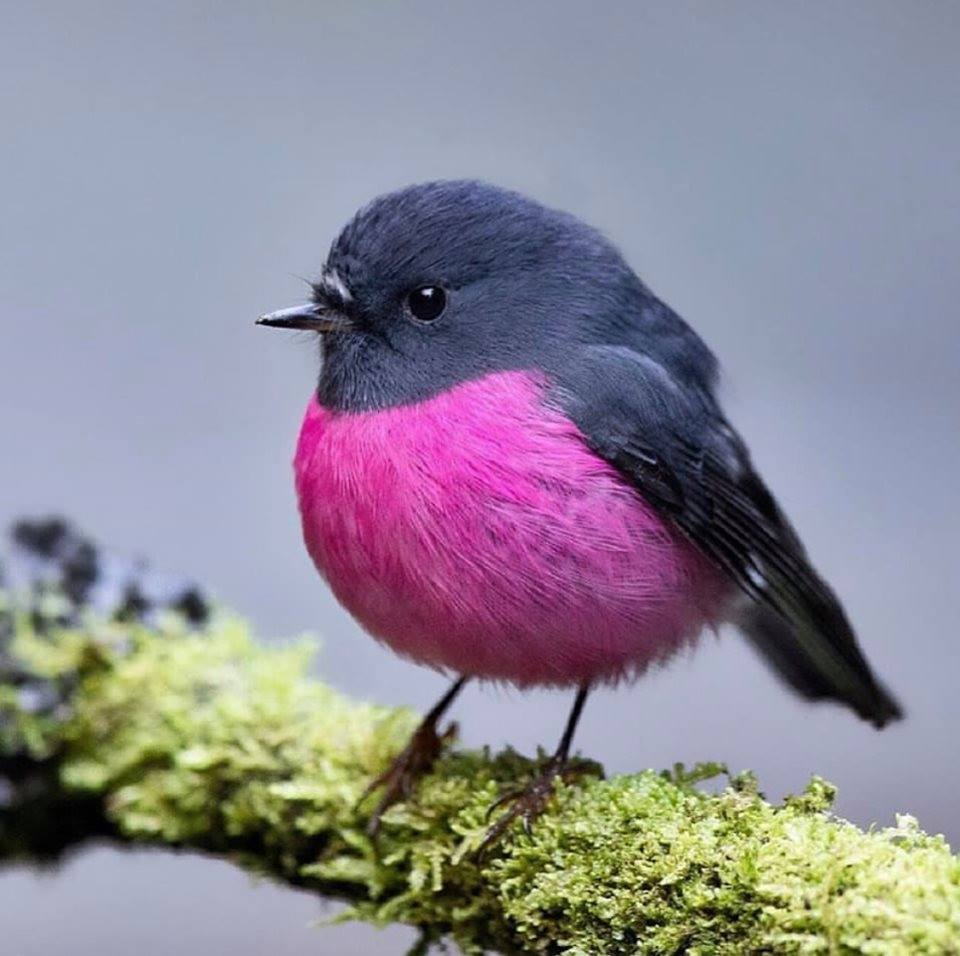
\includegraphics[width=0.5\textwidth]{Pictures/4_WHilaszek.jpg}
    \caption{This bird is a rose robin.}
    \label{fig:ptaszek}
\end{figure}
\vspace{1.0cm}

Table~\ref{tab:ptaszki} represents the life expectancy and flight speed of some birds.

\begin{table}[htbp]
\centering
\begin{tabular}{||c|c|c||}
 \hline
 Ptak & szybkość lotu & długość życia \\ [0.5ex]
 \hline\hline
 Jerzyk & 200km/h & 20 lat \\
 \hline
 Wróbel & 42km/h & 3 lata \\
 \hline
 Gołąb & 60km/h & 6 lat \\
 \hline
 Sroka & 30km/h & 12 lat \\
 \hline
 Kaczka & 65km/h & 5-10 lat \\
 \hline
\end{tabular}
\label{tab:ptaszki}
\caption{That is my table.}
\end{table}
\vspace{0.8cm}

Here is my equation: \[\sqrt{x^2+5}=25\]

And here is my function: $ f(x) = \frac{5}{x} $
\vspace{3.8cm}

My favorite birds:
\begin{enumerate}
    \item Blue tit
    \item Kestrel
    \item Bullfinch
    \item Long-tailed tit
    \item Kinglet
\end{enumerate}

\vspace{0.8cm}

And here are some birds that I don't like:
\begin{itemize}
\renewcommand{\labelitemi}{$-$}
    \item Magpie
    \item Cuckoo
    \item Jaybird
\end{itemize}

\vspace{0.8cm}

\setlength{\parindent}{10ex}
 {\textbf{The cuckoos} are generally medium-sized slender birds. Most species live in trees, though a sizeable minority are ground-dwelling. The family has a cosmopolitan distribution; the majority of species are tropical. Some species are migratory. The cuckoos feed on \underline{insects, insect larvae} and a variety of other animals, as well as fruit. Some species are \textbf{brood parasites, laying their eggs in the nests of other species and giving rise to the metaphor cuckoo's egg}, but the majority of species raise their own young.} \par
 
\setlength{\parindent}{10ex}
 {\emph{Cuckoos have played a role in human culture for thousands of years}, appearing in Greek mythology as sacred to the goddess Hera. In Europe, the cuckoo is associated with spring, and with cuckoldry, for example in Shakespeare's Love's Labour's Lost.\textbf{ In India, cuckoos are sacred to Kamadeva}, the god of desire and longing, whereas in Japan, the cuckoo symbolises \textbf{unrequited} \underline{love}.} \par
 
 





\newpage
\section{Wiktor Prosowicz}{\centering}

My favourite mathematical expression is so called "Piwo equation" : \\
\(P^2 + I*W*O =  :-)\)

\vspace{1cm}
\begin{quote}{\small}
    The most important mathematical thesis can be described as \\
    \(\sqrt{PIWO} + \sqrt{sok} = :-(\) -- Socrates
\end{quote}
\vspace{2cm}

This is my favourite kind of beverage:
\begin{figure}[htbp]
    \centering
    
\includegraphics[scale=0.6]{Pictures/5_WProsowicz_romperek.jpg}
    \caption{Romperek mmmmmm pyszny}
    \label{fig:romper}
\end{figure}
\vspace{1cm}

\setlength{\parindent}{10ex}
 \textbf{ Następny wynalazek grupy CO, dostępny w sieci Żabka. Najprawdopodobniej następca Roger's Strong, szata graficzna puszki ta sama, tylko nazwa piwa zmieniona. Czy to produkt browaru z Brzeska, to sobie głowy uciąć nie dam, bo podany tylko adres warszawski grupy.
Zawartość alk. 6,2% obj., ekstraktu nie podano, cena niecałe 2 złote.
Piana obfita przez krótka chwilę, gaz w normie, jak na stronga, to tej mocy nie czuć. Piwo na \underline{spróbowanie}}.\par
\vspace{0.5cm}

\setlength{\parindent}{10ex}
 \textit{Właśnie popijam Rompera Strong. Zapach lekko chmielowy.Piana zniknęła w mgnieniu oka. Wysycenie całkiem przyzwoite. Barwa jasno miodowa. W smaku czuć alkohol oraz goryczkę. Ogólnie jednak wodnisty. Nie polecam. Moja ocena 2-.}
 \par
\vspace{1.0 cm}

\centering
\begin{table}[htbp]
\centering
\begin{tabular}{|l|l|l|ll}
\cline{1-3}
\cellcolor[HTML]{FFCCC9}{\color[HTML]{333333} \textbf{Nazwa}} & \cellcolor[HTML]{FFCCC9}{\color[HTML]{333333} \textbf{Ocena}} & \cellcolor[HTML]{FFCCC9}{\color[HTML]{333333} \textbf{Cena}} &  &  \\ \cline{1-3}
Romper Extra Strong                                           & 5.0                                                           & 3 zł                                                         &  &  \\ \cline{1-3}
Kuflowe Mocne                                                 & 4.0                                                           & 2.5 zł                                                       &  &  \\ \cline{1-3}
Wódeczka Soplica                                              & 4.5                                                           & 24 zł                                                        &  &  \\ \cline{1-3}
\end{tabular}
\label{tab:piwa}
\end{table}
--Table containing drinks that are always good
\par
\vspace{1cm}

List of project I'm working on
\begin{enumerate}
  \item Flashcard App
  \item HTML Parser
  \item Chinese characters database management app
\end{enumerate}
\vspace{1cm}

List of my planned projects
\begin{itemize}
\renewcommand{\labelitemi}{$*$}
    \item Website
    \item Online game
\end{itemize}
\vspace{1cm}

\raggedleft
Here you can return to my image: Image nr ~\ref{fig:romper} \\
And here to my table: Table nr ~\ref{tab:piwa}



\newpage
\begin{flushleft}
\section{Łukasz Zawadzki}
\label{sec:lzawadzki}

\vspace{0.5cm}

\textbf{Wzory matematyczne i fizyczne:}\\
Wzór na deltę w równaniu kwadratowym:
$ \ \Delta=b^2+4ac \ $\\
Wzór na dylatację czasu:
$ \ \Delta t'= \frac{\Delta t}{\sqrt{1-\frac{v^2}{c^2}}} \ $
\vspace{0.5cm}\\
Tekst testowy \underline{z podkreśleniem}, \textbf{pogrubieniem} oraz \textit{italicą}.\\
\vspace{0.5cm}
Przykładowe języki programowania i ich twórcy

\begin{table}[htbp]
\centering
\begin{tabular}{|c | c|}

\hline
Nazwa & Twórca\\
\hline
C & Dennis Ritchie \\
Java & James Gosling\\
Python & Guido van Rossum\\
\hline
\end{tabular}
\end{table}
\label{tab:Języki}
\vspace{1.0cm}

\begin{figure}[htbp]
    \centering
    
\includegraphics[width=0.5\textwidth]{Pictures/6_LZawadzki.png}
    \caption{Python logo}
    \label{fig:Python_logo}
\end{figure}
\vspace{0.5cm}


Najpopularniejsze systemy operacyjne:
\begin{itemize}
\renewcommand{\labelitemi}{$>$}
    \item Windows
    \item MAC OS
    \item Linux
\end{itemize}
\vspace{0.5cm}
Języki programowania względem popularności:
\begin{enumerate}
    \item Python
    \item C
    \item Java
    \item C++
    \item C\#
    \item Visual Basic
    \item JavaScript
    \item SQL
\end{enumerate}


\vspace{0.5cm}

\textbf{What is Lorem Ipsum?} (tekst z akapitami)\\

\setlength{\parindent}{10ex}
    \par{\underline{Lorem Ipsum} is simply dummy text of the printing and typesetting industry. Lorem Ipsum has been the industry's standard dummy text ever since the 1500s, when an unknown printer took a galley of type and scrambled it to make a type specimen book. It has survived not only five centuries, but also the leap into electronic typesetting, remaining essentially unchanged. It was popularised in the 1960s with the release of Letraset sheets containing \textit{Lorem Ipsum} passages, and more recently with desktop publishing software like Aldus PageMaker including versions of Lorem Ipsum.}\\
\setlength{\parindent}{10ex}
    \par{It is a long established fact that a reader will be distracted by the readable content of a page when looking at its layout. The point of using \textbf{Lorem Ipsum} is that it has a more-or-less normal distribution of letters, as opposed to using 'Content here, content here', making it look like readable English. Many desktop publishing packages and web page editors now use Lorem Ipsum as their default model text, and a search for 'lorem ipsum' will uncover many web sites still in their infancy. Various versions have evolved over the years, sometimes by accident, sometimes on purpose (injected humour and the like).}\vspace{0.5cm}\\
\textbf{Odwołania do:}\\
Figury: \ref{fig:Python_logo}\\
Tabeli: \ref{tab:Języki}
\end{flushleft}


\end{document}
